\documentclass[11pt]{article}
\usepackage[T1]{fontenc}
\usepackage[utf8]{inputenc}
\usepackage{lmodern,microtype}
\usepackage[margin=1in]{geometry}
\usepackage{amsmath,amssymb,amsthm,mathtools,mathrsfs}
\usepackage{graphicx,booktabs,array,enumitem}
\usepackage[round,authoryear]{natbib}
\usepackage{setspace}
\usepackage{xr-hyper}
\usepackage[colorlinks=true,linkcolor=blue,citecolor=blue,urlcolor=blue]{hyperref}
\usepackage{bookmark}
\allowdisplaybreaks
\setlength{\emergencystretch}{2em}
\setlist{topsep=3pt,itemsep=2pt}
\newtheorem{theorem}{Theorem}
\ifdefined\JASASubmission
\newtheorem{proposition}{Proposition}
\newtheorem{lemma}{Lemma}
\newtheorem{corollary}{Corollary}
\else
\newtheorem{proposition}[theorem]{Proposition}
\newtheorem{lemma}[theorem]{Lemma}
\newtheorem{corollary}[theorem]{Corollary}
\fi
\theoremstyle{remark}
\ifdefined\JASASubmission
\newtheorem{remark}{Remark}
\else
\newtheorem{remark}[theorem]{Remark}
\fi
\newcommand{\EE}{\mathbb E}
\newcommand{\PP}{\mathbb P}
\newcommand{\cR}{\mathfrak R}
\newcommand{\cS}{\mathscr S}
\newcommand{\cC}{\mathscr C}
\newcommand{\cN}{\mathcal N}
\newcommand{\ind}{\mathbf 1}
\newcommand{\logp}{\log_+}
\DeclareMathOperator{\kl}{kl}
\DeclareMathOperator{\TV}{TV}
\DeclareMathOperator*{\argmax}{arg\,max}
\DeclareMathOperator*{\argmin}{arg\,min}

\setstretch{1.08}
\externaldocument[][nocite]{manuscript}
\externaldocument[S-][nocite]{supplement}
\renewcommand{\thesection}{C\arabic{section}}
\renewcommand{\thetheorem}{C\arabic{theorem}}
\renewcommand{\theequation}{C\arabic{equation}}
\renewcommand{\thefigure}{C\arabic{figure}}
\renewcommand{\thetable}{C\arabic{table}}
\title{Computational supplement to ``The temporal geometry of bandits with arriving arms''}
\author{}
\date{}
\begin{document}
\maketitle
All risks reported here are expected pseudo-regrets under specified
Bernoulli experiments. Except for the exact finite-prior dynamic
program, estimates use independent Monte Carlo replications; their
standard errors do not quantify uncertainty about a minimax value.
The accompanying scripts save the means, arrival schedules, seeds,
per-replication losses and verification records.
\tableofcontents
\section{Compatible-prior experiments and an exact Bayes benchmark}\label{sec:bayes-experiment-details}
\subsection{The common environment and the schedule comparison}
The multiscale schedules have $k_j=2\cdot4^j$ competitors with lifetime $H_j=T/4^j$. Put $v_j=\sqrt{(k_j-1)/H_j}$ and $\epsilon_j=av_j/32$, where $a\in\{1,4,8\}$. For the simulated ranges $v_j\le1$, consecutive $v_j$ increase by more than a factor of two, and all dyadic exponents have the same parity. Every group is consequently retained by the selection in Section~\ref{S-sec:spectral-proofs} of the mathematical supplement. The reference has mean $\theta_j=1/2+\sum_{r<j}\epsilon_r$. Under the group's null all $k_j-1$ candidates have mean $\theta_j-\epsilon_j$; a spike replaces one such mean by $\theta_j+\epsilon_j$. The null has probability $1/2$ and each spike has probability $1/\{2(k_j-1)\}$. These latent draws are independent across groups. The anchor mean is $1/2$ and unused arms have mean $1/4$.

For each group the largest possible earlier mean is at most $\theta_j$, irrespective of the earlier latent draws. Reference levels are deterministic, so their observations do not reveal other groups' latent variables. In every simulated configuration, including $a=8$, all means are strictly between zero and one. The original lower-bound information calculation applies with $a=1$; the larger multipliers are sensitivity experiments on valid stationary environments, without the same claimed information constant.

The compressed schedule puts the first $2L$ competing labels at time one and all remaining labels at time $T$. Its native prior is constructed by the same selection rule, leaving its last-round arms at mean $1/4$. Each pair has the same label set and tie ordering. At $a=4$, every mean vector from either native prior is evaluated on both schedules. Labels and means remain fixed during this crossing; only arrival times change. Native-prior comparisons and crossed comparisons therefore answer different questions. Other gap multipliers are evaluated only on their native schedules.

Each of the 23,552 trajectories uses a causal policy. MC-MOSS and Cold MC share local clock, frozen capacity, and smallest-label ties; Cold MC alone clears its counts and sums when the competitor count doubles. Both see only observed arrivals and rewards. The simulator supplies one independent uniform variate per calendar round, shared across the two methods and across receiving schedules for a fixed environment. Distinct replications use independent seed sequences. The simulation comprises 591,134,720 policy rounds. Each window is the native testing window of the receiving schedule. Windows are disjoint; their losses and the loss outside their union sum to the full trajectory loss. At $T=65536$, $L=4$ and $a=4$, the four native multiscale windows contribute 3.87, 9.59, 13.75 and 15.39 units of mean MC-MOSS regret, with 104.07 outside their union.

\begin{figure}[tb]
 \centering
 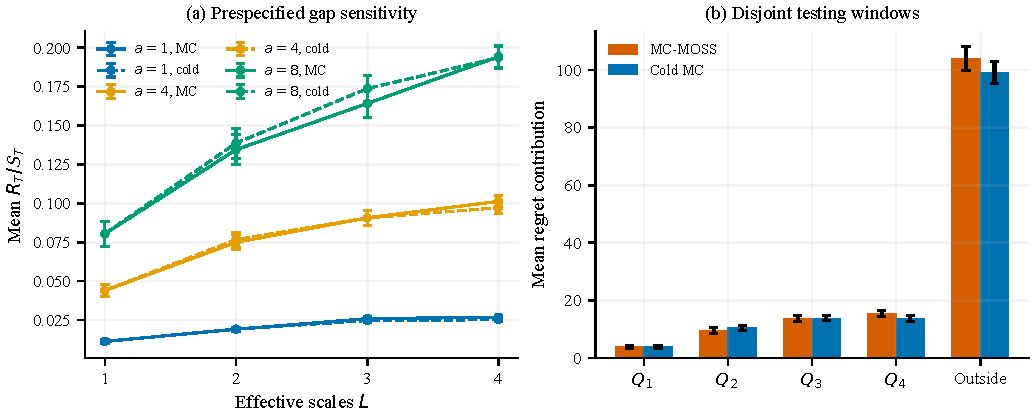
\includegraphics[width=\textwidth]{figures_v2/fig_geometry_sensitivity.pdf}
 \caption{Prespecified sensitivity and window losses at $T=65536$. Left: spectral-normalized native-prior risk for multipliers $a=1,4,8$. Right: regret in the four disjoint testing windows and outside their union for $L=4$, $a=4$. Error bars are $1.96$ Monte Carlo standard errors across 128 independent replications. The proof's small gap constant produces small absolute losses; increasing it changes finite-sample difficulty without changing the spectrum.}
 \label{fig:geometry-sensitivity}
\end{figure}

\subsection{An exact finite-prior dynamic program}
Let $\{\mu^{(e)}:e\in E\}$ be a finite set of Bernoulli mean vectors with strictly positive rational coordinates below one, and let $w_e>0$ be rational prior weights summing to one. The deterministic schedule and this prior are known to the Bayes rule. For every uncertain arm, retain its numbers of successes and failures in a state $s$. Arms whose mean is identical in all environments need not enter $s$. The posterior is
\[
 p_e(s)=\frac{w_e\prod_i (\mu_i^{(e)})^{s_i^+}(1-\mu_i^{(e)})^{s_i^-}}
 {\sum_f w_f\prod_i (\mu_i^{(f)})^{s_i^+}(1-\mu_i^{(f)})^{s_i^-}}.
\]
Action probabilities cancel from the likelihood because the decision rule is the same function of past observations in every environment. This remains true for adaptive sampling. Define
\[
 q_i(s)=\sum_ep_e(s)\mu_i^{(e)},\qquad
 g_t(i,s)=\sum_ep_e(s)\left(\max_{a\in A_t}\mu_a^{(e)}-\mu_i^{(e)}\right).
\]
Write $s^{i,y}$ for the updated state after reward $y$, and leave the state unchanged when $i$ has a known mean. The terminal value is $V_{T+1}=0$, and backward induction gives
\begin{equation}\label{eq:finite-bayes-recursion}
 V_t(s)=\min_{i\in A_t}\{g_t(i,s)+q_i(s)V_{t+1}(s^{i,1})+
       [1-q_i(s)]V_{t+1}(s^{i,0})\}.
\end{equation}

\begin{proposition}\label{prop:exact-finite-bayes}
The recursion \eqref{eq:finite-bayes-recursion} equals the minimum Bayes expected pseudo-regret over all causal policies with the specified information. All its entries are rational, and its initial value is a lower bound for the deterministic-schedule minimax regret over bounded stationary reward laws.
\end{proposition}
\begin{proof}
The posterior is sufficient for prediction because rewards are independent conditional on the environment and the observed counts determine the likelihood. Given the state and selected arm, the next reward is Bernoulli with mean $q_i(s)$, and its conditional expected current regret is $g_t(i,s)$. At the final round minimizing that expectation is optimal. Induction on the number of remaining rounds gives \eqref{eq:finite-bayes-recursion}; randomization cannot improve the minimum of finitely many action values. There are finitely many states with at most $T$ observations, and all posterior denominators are positive. Sums, products, ratios and finite minima of rational numbers remain rational, so exact arithmetic computes the value without rounding an action comparison. Finally, for every policy the supremum over reward laws is at least its average over this finite prior. Taking the infimum over policies proves the lower-bound assertion. Allowing the optimizing policy to use this known prior gives precisely the infimum of that average, not a larger quantity.
\end{proof}

We use six arms with arrivals $(1,1,1,T-1,T-1,T-1)$, for $T\in\{4,6,8,10\}$. Labels in this description start at zero. The anchor and the first reference (labels 0 and 1) have mean $1/2$; label 2 has mean $1/2-\epsilon_1$ or $1/2+\epsilon_1$, with equal probability. Label 3 has mean $1/2+\epsilon_1$. Labels 4 and 5 have common null mean $1/2+\epsilon_1-\epsilon_2$ with probability $1/2$; with probability $1/4$ each, one of them alone has mean $1/2+\epsilon_1+\epsilon_2$. The two latent draws are independent, giving six environments. We set $(\epsilon_1,\epsilon_2)=(1/d,2/d)$ for $d=16,8$. This small example retains the common null/spike structure; it is not an attempt to reproduce all dyadic testing-window conditions at these very short horizons.

All Bellman probabilities, values and comparisons are computed as exact fractions. We independently integrate the returned optimal rule over each environment's complete binary reward tree; the weighted average agrees exactly with the initial Bellman value in all eight cases. The risks of the two implemented anytime policies are computed by the same full reward-tree integration, retaining each policy's full observation history. Their index decisions use the stated numerical implementation. No Monte Carlo approximation enters this benchmark.

\begin{table}[tb]
\centering
\caption{Exact finite-prior risks, displayed to six decimals. The optimal rule knows the prior and complete schedule; MC-MOSS and Cold MC do not. Exact numerators and denominators are supplied with the code.}
\label{tab:exact-bayes}
\begin{tabular}{rr rrr}
\toprule
$T$ & $d$ & Bayes optimum & MC-MOSS & Cold MC\\
\midrule
4 &16&0.183594&0.250000&0.312500\\
6 &16&0.237320&0.311523&0.374023\\
8 &16&0.289612&0.368656&0.431156\\
10&16&0.339413&0.428149&0.490649\\
4 &8 &0.359375&0.500000&0.625000\\
6 &8 &0.449463&0.621094&0.746094\\
8 &8 &0.534172&0.724670&0.849670\\
10&8 &0.610496&0.837447&0.962447\\
\bottomrule
\end{tabular}
\end{table}

\begin{figure}[tb]
 \centering
 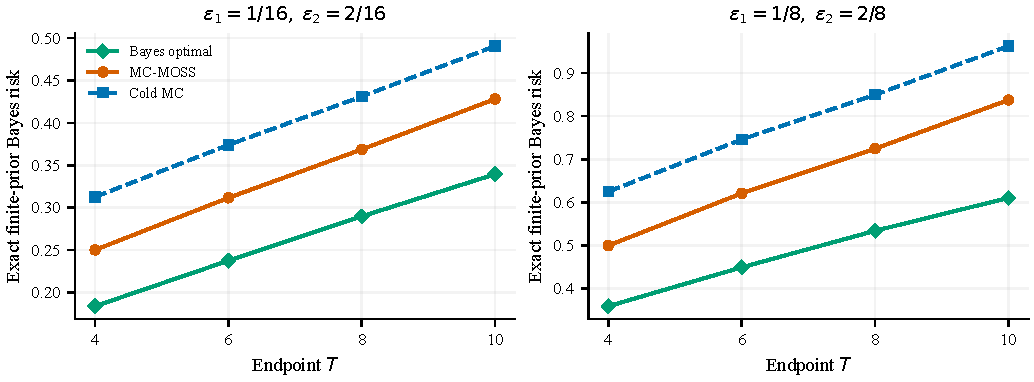
\includegraphics[width=\textwidth]{figures_v2/fig_bayes_exact.pdf}
 \caption{Exact finite-prior Bayes risks for the two gap choices. The green curve is the value of a rule with known schedule and prior. It is a certified lower bound, with no claim that this prior is least favorable. All plotted values are exact rational calculations, so there are no Monte Carlo error bars.}
 \label{fig:bayes-exact}
\end{figure}

\section{Clock, capacity and history interventions}
\subsection{Mechanism experiment: complete specification}
\label{sec:mechanisms-details}

The experiment uses an initial anchor, labeled zero, and 32 candidates
labeled $1,\ldots,32$.  Candidate batches are $1{:}4$, $5{:}8$,
$9{:}16$, $17{:}24$, and $25{:}32$, with arrival times given in the main
text.  The following definitions fix each mean vector before any reward
is simulated:
\begin{enumerate}
\item Near ties: the anchor has mean $0.52$; candidates have mean $0.50$,
except labels $4,8,16,24,32$, which have mean $0.515$.
\item Poor candidates: the anchor has mean $0.70$; candidate $i$ has mean
$0.10+0.05(i\bmod 4)$.
\item New record: the anchor has mean $0.45$; candidates have mean $0.35$,
except label $17$, which arrives at $\lfloor T/2\rfloor+1$ with mean $0.80$.
\item Mixed late batch: the anchor has mean $0.55$ and the first 24
candidates have mean $0.40$.  The last batch has means
$(0.15,0.35,0.52,0.58,0.62,0.72,0.48,0.20)$.
\item Near upper bound: the anchor has mean exactly one; candidates have
mean $0.94$, except labels $4,8,16,24,32$, which have mean $0.985$.
\end{enumerate}
In the reverse-order version, the reward distributions remain attached
to the same physical arms; only their positions within each candidate
batch change.  All index rules choose the first label among maximizers.
For the confidence-index rules, unobserved arms have infinite index,
except for clipped MC-MOSS, for which the index is one.
Thompson sampling instead draws independently from
$\operatorname{Beta}(1+S_i,1+N_i-S_i)$ for every present arm at each
decision.  An arriving arm begins with $N_i=S_i=0$, and none of these
baselines discards observations.  KL-UCB uses
\[
 U_i(t)=\sup\{q\in[\widehat\mu_i,1]:
 N_i\operatorname{kl}(\widehat\mu_i,q)\leq\log t\}.
\]
The scalar root is computed by 32 bisections, with an index error below
$2^{-32}$.  A monotonicity check skips a root only when its exact index
cannot exceed the current maximizer.  Neither the horizon, the means,
nor unrevealed arrivals enter any decision function.

There are $5\times2\times2\times128\times10=25{,}600$ trajectories and
$131{,}072{,}000$ policy rounds.  The seed for reward uniforms is
$73061013+10^6h+10^4c+r$, where $h,c,r$ are zero-based horizon,
configuration, and replication indices.  The Thompson stream adds
$5\times10^6$.  The two label orders use the same seeds.  The development
run instead starts at seed $41061013$ and uses two replications per cell;
its role is software validation, with no tuning or selection of parameters.
The paired standard error of a contrast is its sample standard deviation
over replications divided by $\sqrt{128}$.  Every plotted interval is
pointwise, without simultaneous-coverage interpretation.

\begin{figure}[p]
\centering
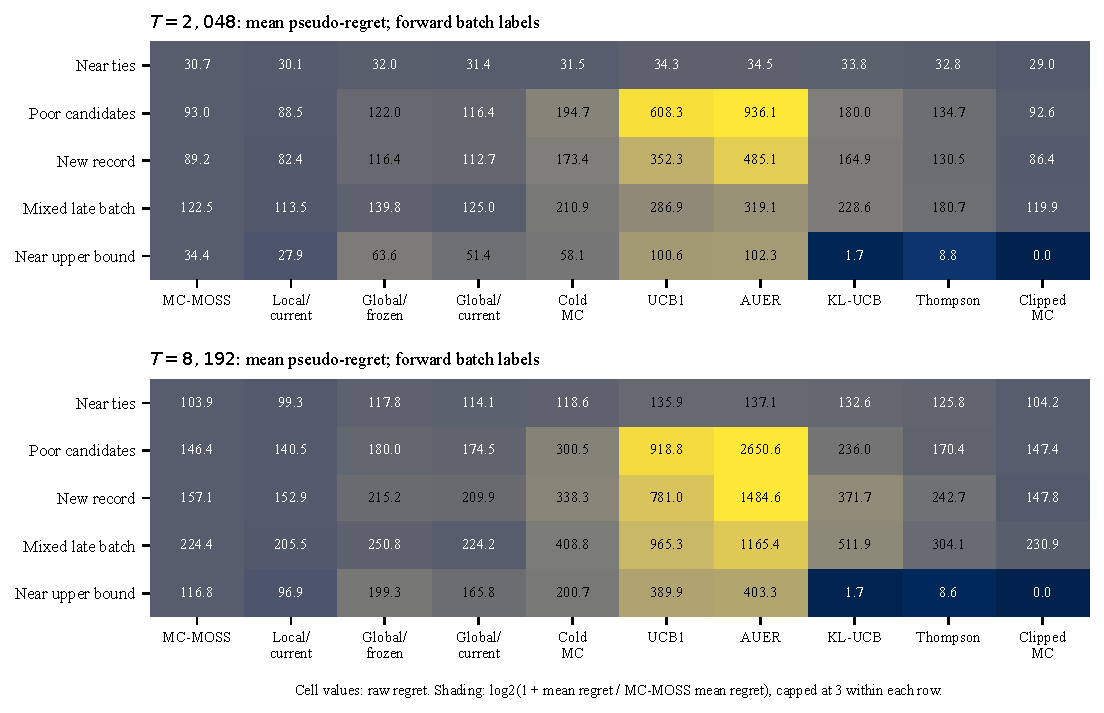
\includegraphics[width=\linewidth]{figures_v2/fig_mechanisms_baselines.pdf}
\caption{Complete forward-label mean pseudo-regrets for both horizons.
Numbers report raw regret.  Color encodes
$\log_2(1+\overline R_{\rm method}/\overline R_{\rm MC})$, capped at three
for display, within each row; it does not encode sampling uncertainty.
The tables in the released CSV files give Monte Carlo standard errors
and the reverse-label results for every cell.  The exact boundary anchor
explains the zero for the clipped rule in the last row.}
\label{fig:mechanisms-baselines-all}
\end{figure}

\begin{figure}[p]
\centering
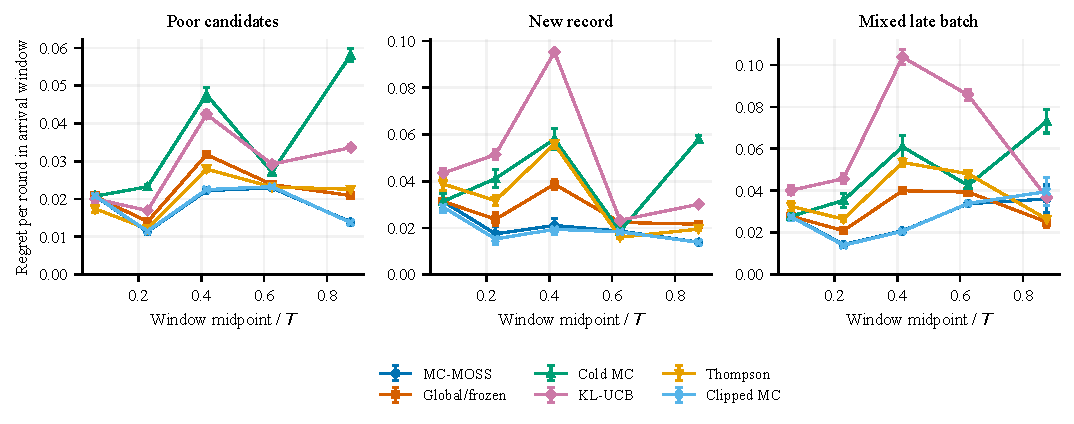
\includegraphics[width=\linewidth]{figures_v2/fig_mechanisms_windows.pdf}
\caption{Mean regret per round in the five intervals between consecutive
batch arrivals, at $T=8192$ with forward labels.  Bars are $1.96$ Monte
Carlo standard errors.  In the new-record configuration the fourth
interval begins with the arrival of the arm of mean $0.80$; in the mixed
configuration the fifth interval begins with the last heterogeneous
batch.  Window midpoints indicate the horizontal positions; connecting
segments are guides to the eye.}
\label{fig:mechanisms-windows}
\end{figure}

The software audit compared 2,316 MC-MOSS and cold-reset decisions with
the original online implementation.  It also checked 60 prefixes after
removing all future arm labels, 60 exact reruns, 800 direct evaluations of
the factorial index formulas, and 189 KL roots against an independent
Brent solver.  The largest root discrepancy was $9.37\times10^{-11}$.
Three posterior-moment checks used $10^5$ beta draws each.  These checks
validate the implementation and its information restrictions; they do
not establish regret guarantees for the experimental baselines.

\section{Random-arrival experiments}
\subsection{Common-gap selection and independent evaluation}
The two-arm experiment uses the designs in Section~\ref{sec:experiment-random}.
Each conditional cell fixes $T,H,\Delta$ and the sign before drawing
rewards. If $n_0=T-H$, the sole anchor's sufficient statistics at the
first competitor arrival are $(N_0,S_0)=(n_0,\operatorname{Bin}(n_0,1/2))$.
This compression has exactly the same law as the full forced prefix.
MC-MOSS uses these statistics and a local clock starting at one;
Fresh-H MOSS discards them and uses the fixed remaining horizon $H$.
Both indices have the form
$\widehat\mu_i+\sqrt{[\log\{u/(2N_i)\}]_+/N_i}$,
with $u=s$ at the $s$th post-arrival decision for MC-MOSS and $u=H$
for Fresh-H MOSS. Unobserved arms have infinite index, and ties favor
the anchor. A shared independent uniform variate at each decision
couples the two methods' rewards within a replication.

Development and held-out strata use 64 and 128 replications. The seed
of stratum $(m,j,e)$ is
$2026101303+o+100000m+1000j+e$, where $e$ indexes the gap/sign grid
and $o=0$ for development and $o=10000000$ for evaluation.
All seeds in these two sets are distinct. For each method and arrival
law, development means select either one common grid member or one
member for every $H$. Only the former defines a lawful reward
environment fixed before the random schedule. The latter is a
schedule-dependent benchmark. Different methods may select different
environments, so their displayed selected risks are not a paired
comparison under one common environment.

For selected stratum losses $R_{jr}$ and known probabilities $p_j$, the
reported estimate and standard error are
\[
 \widehat r=\sum_jp_j\overline R_j,\qquad
 \widehat{\operatorname{se}}(\widehat r)
 =\left\{\sum_jp_j^2s_j^2/128\right\}^{1/2},
\]
where $s_j^2$ is the unbiased sample variance. Independent strata
justify this expression. Conditional on the development selections,
these are unbiased estimates of the selected environments' risks.
They are not unbiased estimates of a maximum over the grid.

The additional direct-draw experiment samples 2048 lifetimes from each
arrival law, keeps its development-selected common environment fixed,
and generates new rewards. It has its own random stream. Its ordinary
Monte Carlo standard error includes both arrival and reward variation.
The two estimates in Table~\ref{tab:random-selected} therefore need not
coincide. All endpoints, selected indices, gap values, signs and seeds
are saved in the released CSV and compressed raw arrays.

\begin{table}[tb]
\centering\small
\caption{Selected-environment risks at $T=16384$. Parentheses are
Monte Carlo standard errors. ``Specific'' permits the development
environment to depend on the realized schedule. ``Direct common''
uses 2048 new random schedules under the common environment.}
\label{tab:random-selected}
\begin{tabular}{llrrr}\toprule
Arrival law & Policy & Common & Specific & Direct common\\\midrule
Inverse square root & Fresh-H & 1.321 (0.018) & 1.977 (0.026) & 1.319 (0.053) \\
Inverse square root & MC & 1.384 (0.000) & 1.781 (0.020) & 1.302 (0.035) \\
Uniform scales & Fresh-H & 13.339 (0.440) & 14.768 (0.399) & 12.139 (0.529) \\
Uniform scales & MC & 11.262 (0.366) & 13.459 (0.398) & 11.377 (0.458) \\
Short concentrated & Fresh-H & 0.675 (0.006) & 0.738 (0.005) & 0.667 (0.014) \\
Short concentrated & MC & 0.721 (0.000) & 0.731 (0.002) & 0.711 (0.014) \\
Two longest scales & Fresh-H & 47.389 (1.753) & 43.332 (1.546) & 45.121 (0.698) \\
Two longest scales & MC & 41.920 (1.420) & 40.544 (1.554) & 39.202 (0.648) \\
Longest scale & Fresh-H & 57.365 (2.771) & 57.365 (2.771) & 60.868 (0.717) \\
Longest scale & MC & 57.818 (2.921) & 57.818 (2.921) & 57.591 (0.742) \\
\bottomrule\end{tabular}
\end{table}

\begin{figure}[p]\centering
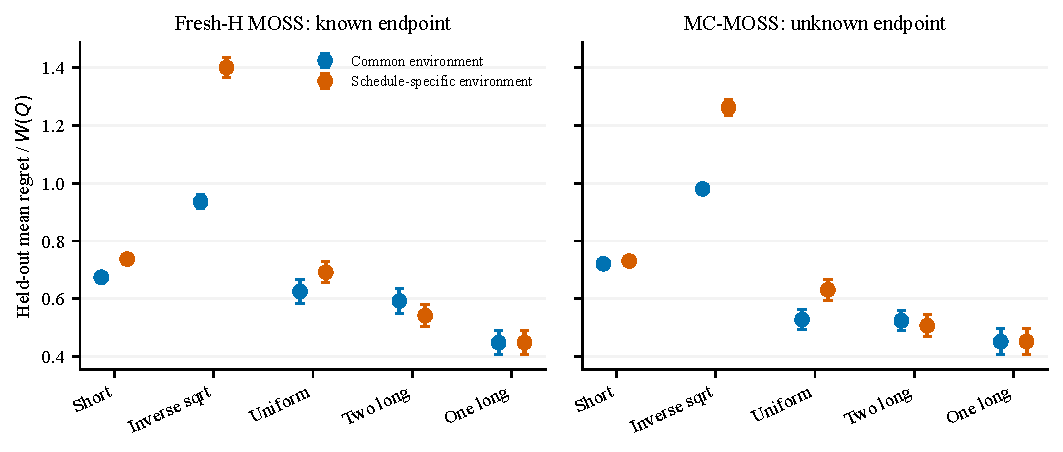
\includegraphics[width=\linewidth]{figures_v2/random_mixture_comparison.pdf}
\caption{Held-out common and schedule-specific selected risks at
$T=16384$ for all five arrival laws, divided by $W(Q)$. Bars are
$1.96$ stratified Monte Carlo standard errors. Selection takes place
on an independent finite development sample, so the held-out
ordering need not agree with the order of exact grid maxima.}
\label{fig:random-mixtures}
\end{figure}

The full study executes 451,072 policy trajectories and 687,147,832
post-arrival policy decisions, including development, held-out and
direct-draw runs. The zero-regret forced prefixes are compressed as
described above. Independent verification replays 1,008 conditional
trajectories and reconstructs all 2,992 grid summaries and all 80
selected held-out summaries from the raw arrays.

\subsection{The two-batch stretch implementation}
Section~\ref{sec:stretch-experiment} specifies the fixed template and
common mean vectors. Before the first batch, the count is $T-4H$ and
the anchor's success count is drawn from $\operatorname{Bin}(T-4H,1/2)$.
At the first arrival, the informed rule infers $H$ from $T$ and the
observed time and runs fresh MOSS for $3H$ rounds on three arms.
At the second arrival it runs fresh MOSS for $H$ rounds on five arms.
MC-MOSS retains all prefix and intermediate observations. Every loss
after the first batch is recorded, including the complete $3H$ prefix
before the final batch.

The development and held-out base seeds are 841013 and 951013; the
stratum seed adds $100000m+1000j+r$. The sets are disjoint over the
simulated indices. Both methods and all grid members share the reward
uniforms for a fixed stratum and replication. Development selects one
environment for each $(m,Q)$ using the informed rule's risk. Both rules
then face that same environment at every stretch in evaluation.
Unlike Table~\ref{tab:random-selected}, this is a common-environment
comparison across methods; it does not separately maximize MC-MOSS's
risk over the grid.

The 84,480 stratum trajectories require 111,390,720 post-first-arrival
policy decisions. Nine full-calendar comparisons verify the prefix
compression against the original MC implementation. The saved-data
audit checks every interval-loss decomposition, all 12 development
selections and all 24 held-out summaries. Complexity curves are
computed independently of rewards; the capacity calculation agrees
with $2\sqrt{3H/2}+2\min\{H/2,\sqrt{H/2}\}$.

\section{The earlier fixed-endpoint study}\label{sec:earlier-experiments}

The experiments examine three distinct questions: whether the geometric
quantities distinguish arrival schedules with the same final arm count;
whether retaining observations avoids repeated exploration after a clock
reset; and how the proposed rule behaves on several finite Bernoulli
instances. They do not estimate minimax risk, which involves a supremum
over reward environments.

\subsection{Design and implementation}

We use $T=16{,}384$ rounds and $K_T=86$ arms, with an anchor present at
time one. The early-batch schedule makes all 85 competitors available at
time one. The late-batch schedule introduces them at $T-255$. The regular
schedule places their arrivals at the 85 integer times
$\lfloor 1+q(T-256)/84\rfloor$, $q=0,\ldots,84$.
The multiscale schedule uses batches of sizes $1,4,16,64$ with remaining
lifetimes $T,T/4,T/16,T/64$, respectively. Arm labels follow arrival
order; this order also resolves index ties.

Each schedule is crossed with two fixed mean vectors. In the persistent
incumbent configuration, the anchor has mean $0.6$ and every competitor
has mean $0.5$. In the improving-record configuration, all arms have
mean $0.4$ except competitor labels $1,22,43,85$, whose means are
$0.45,0.50,0.55,0.60$. The same labeled mean vector is used across
schedules. Thus the early and late batches contain the same candidates,
while the regular and multiscale schedules expose new record means over
time. Rewards are Bernoulli and conditionally independent of the past
given the selected arm.

We compare MC-MOSS with three explicitly specified rules. Cold MOSS
uses the same index and clock-reset times as MC-MOSS, but discards all
counts and reward sums at each reset. Full-history UCB uses
$\widehat\mu_i+\sqrt{2\log t/N_i}$, the UCB1 index of
\citet{auer2002finite}, with infinite index for an unobserved arm.
The global-clock MOSS comparison uses
\[
 \widehat\mu_i+
 \sqrt{\frac{[\log\{t/(2(K_t-1)N_i)\}]_+}{N_i}}
\]
whenever $K_t>1$, retains every observation, and does not reset its
clock. This comparison changes both the clock and capacity calibration; we make
no arrival-spectrum guarantee for it. All four policies select the
sole available arm when $K_t=1$. All tuning constants are fixed before
simulation.

There are 256 independent replications per schedule and mean vector.
Within a replication, the methods use the same independent uniform
draw at each calendar time to generate their selected Bernoulli
reward. The resulting coupling permits paired Monte Carlo comparisons;
each policy receives only its own observed reward. Decision functions
receive the current available set, time, counts, and reward sums.
They receive neither the evaluation horizon, future arrivals, nor true
means. We record pseudo-regret relative to the best currently available
mean. Parentheses in Table~\ref{tab:regret} are Monte Carlo standard
errors, computed across replications, rather than reward standard
deviations.

\begin{table}[t]
\centering
\caption{Arrival geometry at the common horizon $T=16{,}384$ with
$K_T=86$. These quantities are computed from arrival times only.}
\label{tab:geometry}
\small
\begin{tabular}{lrrrrr}
\toprule
Arrival schedule & $\mathscr S_T$ & $\mathscr C_T$ & $\Gamma_T$ & $Q_T$ & $D_T^{\rm eff}$ \\
\midrule
Early batch & 1180.10 & 1180.10 & 1181.00 & 1180.10 & 1.00 \\
Late batch & 147.51 & 147.51 & 148.00 & 147.51 & 1.00 \\
Regular arrivals & 1661.63 & 1180.10 & 840.00 & 967.31 & 2.95 \\
Multiscale arrivals & 512.00 & 460.55 & 256.00 & 256.00 & 4.00 \\
\bottomrule
\end{tabular}

\end{table}

\begin{table}[t]
\centering
\caption{Mean pseudo-regret over 256 replications, with Monte Carlo
standard errors in parentheses. ``Incumbent'' and ``Records'' denote
the two fixed mean configurations described in the text.}
\label{tab:regret}
\small
\setlength{\tabcolsep}{3pt}
\resizebox{\textwidth}{!}{\begin{tabular}{llrrrr}
\toprule
Mean configuration & Arrival schedule & MC-MOSS & Cold MOSS & UCB & Global MOSS \\
\midrule
Incumbent & Early batch & 745.6 (23.05) & 745.6 (23.05) & 1599.9 (0.52) & 745.6 (23.05) \\
Incumbent & Late batch & 25.3 (0.06) & 24.8 (0.08) & 25.6 (0.00) & 25.6 (0.00) \\
Incumbent & Regular arrivals & 429.4 (12.71) & 1130.2 (9.28) & 1597.6 (0.60) & 499.0 (12.82) \\
Incumbent & Multiscale arrivals & 123.1 (1.16) & 176.0 (2.27) & 503.1 (1.43) & 211.0 (1.48) \\
\addlinespace
Records & Early batch & 678.9 (18.90) & 678.9 (18.90) & 2938.3 (2.55) & 678.9 (18.90) \\
Records & Late batch & 47.1 (0.31) & 46.5 (0.33) & 49.5 (0.01) & 49.5 (0.02) \\
Records & Regular arrivals & 559.3 (11.54) & 1009.7 (9.69) & 1670.6 (1.36) & 620.1 (11.38) \\
Records & Multiscale arrivals & 140.7 (1.67) & 186.5 (2.52) & 349.8 (1.64) & 220.2 (2.05) \\
\bottomrule
\end{tabular}
}
\end{table}

\subsection{Geometric and finite-sample behavior}

Table~\ref{tab:geometry} shows substantial variation in the spectrum at
fixed $T$ and $K_T$. Moving the common batch from time one to the last
256 rounds divides both the spectrum and the grid-free capacity by
eight. For the multiscale schedule, the four spectral components each
equal 128, so $\mathscr S_T=512$, $Q_T=256$, and
$D_T^{\rm eff}=4$. The regular and early-batch schedules have equal
capacity in this particular construction, although their dyadic
spectra differ. Constant-factor equivalence does not imply equality
of the two functionals.

\begin{figure}[t]
\centering
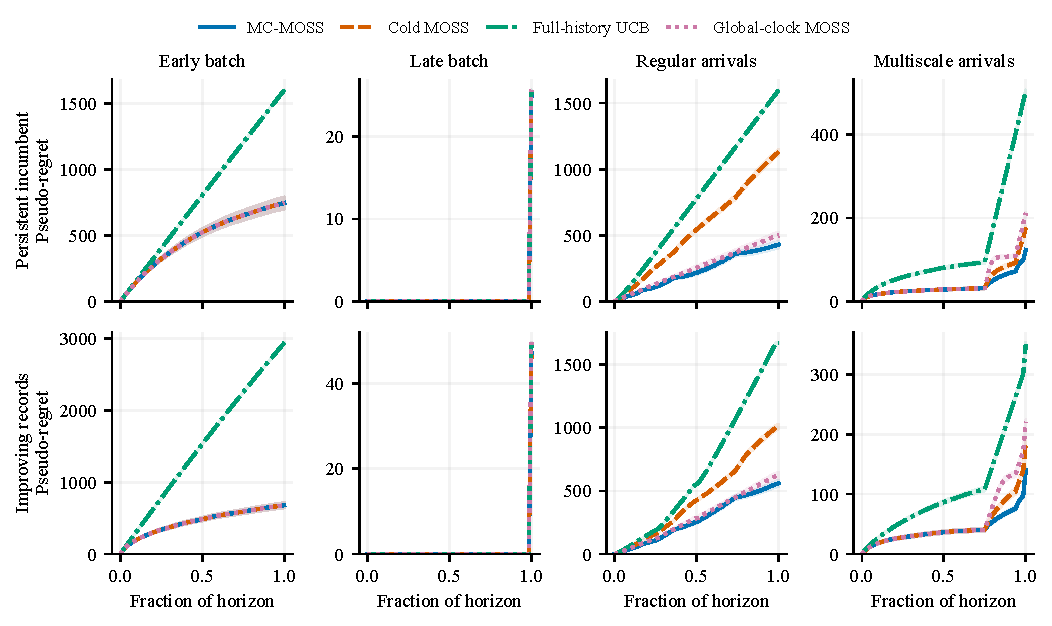
\includegraphics[width=\textwidth]{figures/fig_policy_comparison.pdf}
\caption{Mean cumulative pseudo-regret for the eight Bernoulli
environments. Shaded bands are the mean plus or minus 1.96 pointwise
Monte Carlo standard errors; they are not simultaneous confidence
bands. The first, second, and fourth methods coincide in the
early-batch panels. Vertical scales differ between panels.}
\label{fig:policy-comparison}
\end{figure}

Table~\ref{tab:regret} and Figure~\ref{fig:policy-comparison} show that history retention matters in the regular and multiscale schedules. For regular arrivals with a persistent incumbent, MC-MOSS has mean regret 429.4, compared with 1130.2 for Cold MOSS. The paired mean reduction is 700.8 with Monte Carlo standard error 14.9. MC-MOSS also has lower regret than the global/current comparison in these two schedules. That comparison changes both the clock and capacity calibration, so it does not isolate either effect. When every competitor arrives at time one, the three MOSS rules make identical decisions. The late-batch example gives a counterpoint: with a persistent incumbent, Cold MOSS has mean regret 24.83, versus 25.34 for MC-MOSS. The paired Cold-minus-MC difference is -0.51 with standard error 0.11. History retention therefore does not yield pointwise dominance, even in this small comparison.


These comparisons concern the specified environments and constants.
In particular, the fixed-gap environments need not be least favorable
for any schedule, and a small observed ratio of regret to
$\mathscr S_T$ does not estimate a minimax constant. The UCB comparison
also does not isolate history retention: UCB retains history but uses
a different exploration bonus.

\subsection{Restart costs and reproducibility checks}

We separately reproduce the deterministic restart example using
segment length $h=65{,}536$ and $m=1,\ldots,7$ segments. The first two
arms have rewards $1/2$ and $1/4$; segment $j=1,\ldots,m-1$ adds
$2^{j-1}$ arms with reward $1/2$. MC-MOSS pulls the unique inferior arm
94 times for every reported $m$, giving regret 23.5. Cold MOSS pulls it
94, 179, 255, 322, 380, 429, and 470 times, respectively; its regret
therefore reaches 117.5 at $m=7$. Figure~\ref{fig:structural-diagnostics}(a)
shows this finite repeated-exploration effect. These runs hold $h$
fixed; they do not numerically establish the asymptotic separation
proved using $h=2^{16m}$. The released analytic-bound table evaluates
the proved bounds for that latter family and labels those values as
bounds, not simulated trajectories.

\begin{figure}[t]
\centering
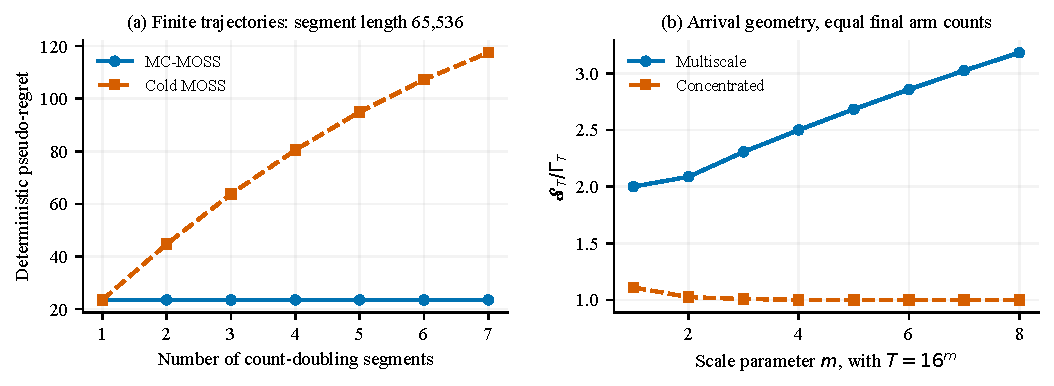
\includegraphics[width=\textwidth]{figures/fig_structural_diagnostics.pdf}
\caption{Two structural diagnostics. (a) Actual deterministic policy
trajectories with fixed segment length. (b) Exact geometric
calculations for the multiscale family with $T=16^m$ and a comparison
schedule with the same final arm count: $m+1$ competitors arrive at
time one and the rest arrive at time $T$. No policy simulation at
these exponential horizons is used in panel (b).}
\label{fig:structural-diagnostics}
\end{figure}

The computational audit also repeats 1,715 exhaustive small schedules
and 10,000 random schedules, checking capacity feasibility, primal--dual
agreement, spectral comparisons, clock charging, and the compatible
scale selection inequalities. An additional 2,001 online API steps
check the original interface and reward-range clipping example. Our
simulation implementation agrees with the original online MC-MOSS
interface on 6,168 individual actions. Forty-eight prefix checks hide
all labels arriving after the shorter endpoint and reproduce every
action on the common prefix for all four policies. The released
scripts, environment tables, seeds, raw replication results, paired
differences, and figure code permit regeneration of all numerical
claims above. These checks support reproducibility and implementation
consistency; the general statements rely on their analytic proofs.

\bibliographystyle{plainnat}
\bibliography{references}
\end{document}
